\newpage
\section{Particle characterization and particle tracking using interference properties}
		\label{sec:chapter2}

\subsection{Introduction}

Properties of coherent light to produce interferences is widely used in metrology for a long time with, for example, the famous Fabry-Pérot  \cite{fabry_theorie_1899, perot_application_1899} and Michelson interferometers \cite{michelson_relative_1887}. The latter was initially used to measure earth's rotation and is still used today, in particular, for the recent measurement of gravitational waves
\cite{ligo_scientific_collaboration_and_virgo_collaboration_gw151226_2016}. 
Since the beginning of the century, interest on tracking and characterizing colloidal particles risen thanks to the democratization of micro fluidics and lab-on-a-chip technologies. In the following I will provide some insights on the three most used :

\begin{itemize}
	\item Reflection Interference Contrast Microscopy (\gls{RICM})
	\item Lorenz-Mie fit
	\item Rayleigh-Sommerfeld back-propagation
\end{itemize}

The first one, \gls{RICM}, uses the principle of optical difference path as a Michelson interferometer. The other two, uses the interference between the light scattered by the colloid and the incident light. Generaly, both of the sources  thuare colinear, wes speak of in-line holography. 

\subsection{In-line holographic video microscopy theory}

\subsubsection{Reflection Interference Contrast Microscopy}

\begin{figure}[h]
	\centering
	\includegraphics[scale=0.8]{02_body/chapter2/images/RICM.png}
	\caption{Figure from \cite{davies_elastohydrodynamic_2018} representing \gls{RICM} with two wavelengths. (a) Left: interference patterns created with a wavelength $\lambda_1 = 532$ nm (scale bar $ 5~\mathrm{\mu m}$). 
		Right: radial intensity profile (black dots) extracted from the image, azimuthally averaged (magenta line) and fitted with Eq.\ref{Eq.RICM} to measure the height of the particle (here $h$). (b) Same as (a) with a wavelength $\lambda_2 = 635$ nm. (c) Time series of the height of a particle $h$ (green: $ \lambda_1$, magenta: $\lambda_2$) and the particle velocity measured along the flow in blue. }
	\label{fig.RICM}
\end{figure}


Reflection Interference Contrast Microscopy was first introduced in cell biology by Curtis to study embryonic chick heart fibroblast \cite{curtis_mechanism_1964} in 1964. \gls{RICM} gained in popularity 40 years after both in biology and physics \cite{filler_reflection_2000, siver_use_2000, weber_2_2003, limozin_quantitative_2009, nadal_probing_2002, raedler_measurement_1992}. It was also used recently in soft matter physics to study elastohydrodynamic lift at a soft wall \cite{davies_elastohydrodynamic_2018}.

When we illuminate a colloid with a plane wave from the bottom, a part of the light is reflected at the surface of the glass substrate and at the colloid's surface. The difference of optical path between the the two reflection create interference parterns. Let's take an interest at the mathematical description of this phenomenon. In the far field, we can describe two different one-dimensional electric field vectors of the same pulsation $\omega$ \cite{f_bohren_absorption_1998} as:

\begin{equation}
	\vec{E}_1(\vec{r}, t) = \vec{E}_{0_1} \cos(\vec{k}_1 \cdot \vec{r} - \omega t + \epsilon_1) ~,
\end{equation}
and
\begin{equation}
	\vec{E}_2(\vec{r}, t) = \vec{E}_{0_2} \cos (\vec{k}_2 \cdot \vec{r} - \omega t + \epsilon_2) ~.
\end{equation}


\nomenclature{$\vec{E}$}{Electrical field}
\nomenclature{$k$}{Wave number}
\nomenclature{$\omega$}{Pulsation}

Where the $k$ is the wave number $k=2\pi n_{\mathrm{m}}/\lambda$, $\lambda$ denoting the illumination wavelength, $n_\mathrm{m}$ the optical index of the medium, $\epsilon_{1,2}$ the initial phase of each waves and $\vec{r}$ the position from the source. Here, the origin ($\vec{r} = \vec{0}$) could be taken at the position of the first reflection (on the glass slide) thus at the particule, $\vec{r}$ would be given by the particle's height such that $|r| = z$ the particle-subtract distance. Experimentaly, we measure the intensity of the interference parttens, those can be computed from the time averaged squared sum of the eletric field $\vec{E} = \vec{E}_1 + \vec{E}_2$. The measured intensity is thus given by:

\begin{equation}
	\begin{aligned}
		I & = \langle \vec{E}^2 \rangle = \langle \vec{E}_1^2 + \vec{E}_2^2 + 2\vec{E}_1 \cdot \vec{E}_2 \rangle 
		= \langle \vec{E}_1^2 \rangle + \langle \vec{E}_2^2 \rangle  + 2 \langle \vec{E}_1 \cdot \vec{E}_2 \rangle \\
		& = \frac{{E_{0_1}^2}}{2} + \frac{{E_{0_2}^2}}{2} +  2 \langle \vec{E}_1 \cdot \vec{E}_2 \rangle ~,
	\end{aligned}
\end{equation} 

where $ \langle \vec{E_1} \rangle $ and  $\langle \vec{E_2} \rangle$ are respectively given by $I_1$ and $I_2$, the incident light intensities. Using the trigonometric formula $2 \cos (a)\cos (b) = \cos (a+b) \cos (a-b) $ we have:

\begin{equation}
	\langle  
	\vec{E}_1 \cdot \vec{E}_2 \rangle = 
	\langle
	\frac{1}{2} \vec{E}_{0_1}  \vec{E}_{0_2} 
	\left[
		\cos 
		\left(
			\vec{k}_1 \cdot \vec{r} - \vec{k}_1 \cdot \vec{r} + \phi	
		\right)	
		+ 
		\cos
		\left(
			2\omega t + \phi'
		\right)
	\right]
	\rangle~.
\end{equation}

As we average over the time, the second $\cos$ will vanish since in general $\langle \cos(at + b) \rangle_ t = 0$ thus:

\begin{equation}
	\langle \vec{E}_1 \cdot \vec{E}_2 \rangle = \frac{1}{2} \langle  \vec{E}_{0_1}  \vec{E}_{0_2} \rangle
	\cos 
	\left(
	\vec{k}_1 \cdot \vec{r} - \vec{k}_2 \cdot \vec{r} + \phi	
	\right)	
\end{equation}

with $\phi$ the phase difference between the two fields, which is generaly equal to $\pi$ due to the reflection properties on a higher index. Indeed a colloid has generaly a greater optical index than the dillution medium.  finaly, the total intensity can be read as:


\begin{equation}
	I = I_1 + I_2 + 2 \sqrt{I_1 I_2} 
	\cos 
	\left(
	\vec{k}_1 \cdot \vec{r} - \vec{k}_2 \cdot \vec{r} + \phi	
	\right)
\end{equation}

By taking $k_1 = - k_2$ due to the reflection properties, we have:


\begin{equation}
	I = I_1 + I_2 + 2 \sqrt{I_1 I_2} 
	\cos 
	\left(
	\frac{4 \pi n_{\mathrm{m}}}{\lambda} z + \phi	
	\right)
\end{equation}


If we now suppose that we have a spherical particle at a height $z$ we can develop the radial interference intensity $I(x)$ as \cite{ raedler_measurement_1992}:

\begin{equation}
	I(x) = A_0 + A_1 \mathrm{e}^{-b_1 x^2} + A_2^{-b_2 x^2} \cos \left[ \frac{4\pi n_m}{\lambda}\left( g(x) + z \right) + \phi \right]
	\label{Eq.RICM}
\end{equation}

Where $A_i$ and $b_i$ are fit parameters and $g(x)$ donotes the contour of the sphere.
Finally, this method is great because the equation are computationaly light and permits to have a quick tracking of particles. However, as we can see on Eq.\ref{Eq.RICM}, due to the periodicity of the cosinus, the interference pattern will be the same for all heights $z$ separated by a distance $\lambda / 2n_\mathrm{m} \approx 200 $ nm (for $\lambda = 532$ nm and $n_{\mathrm{m}} = 1.33$). It is possible to extend this limitation by using 2 differents wavelength to $\approx 1.2 ~ \mathrm{\mu m}$ as used in \cite{davies_elastohydrodynamic_2018}. Despite the precision of this method which can reach the $10$ nm spatial resolution on the particle position measurement, the range limitation is not compatible with the study of $ <5 ~ \mathrm{\mu m}$ particle's Brownian motion making \gls{RICM} not usable for our context since we need at minimum a $5~\mathrm{\mu m}$ of spatial extension on the height measurement.



\subsubsection{Lorenz-Mie Fit}
\label{chap:LM_fit}

A way hologram, is to look at the superimposition of the scattered field $\vec{E}_s$ and incident field $\vec{E}_0$. This way, we could track and characterize even small particles. This method is has been developed in the early 2000 \cite{ovryn_imaging_2000, lee_characterizing_2007}. Since, a lot of studies has been realised with this method. 

Let's the incident field be a plane wave uniformly polarized along the axis $ \hat{e}$, with an amplitude $E_0$ and propagating along the $z$ direction :
\begin{equation}
	\vec{E}_0(\vec{r},z) = E_0(\vec{r}) \mathrm{e}^{ikz}\hat{e}
\end{equation}

Let's consider a particle of radius $a$ at a position $\vec{r}_p $, the scattered field can be written using the Lorenz-Mie theory \cite{f_bohren_absorption_1998} as:

\begin{equation}
	\vec{E}_s(\vec{r}) =  \vec{f}_s(k(\vec{r} - \vec{r}_p))E_0(\vec{r}) \exp \left(-ikz\right) 
\end{equation} 

With $\vec{f}_s$ the Lorenz-Mie scattering function \cite{f_bohren_absorption_1998}. The intensity $I$ that we measure at $\vec{r}$ is given by the super imposition of incident and scattered waves. Since the measurements are done at the focal plane, $I$ is given by:

\begin{equation}
	\begin{aligned}
	I(\vec{r}) & = |\vec{E}_s(\vec{r}, 0) + \vec{E}_0(\vec{r}, 0)|^2 \\
	& = E_0^2(\vec{r}) + 2 E_0^2\operatorname{Re} \left(\vec{f}_s(k(\vec{r}- \vec{r}_p)) \hat{e}\right) + | \vec{f}_s(k(\vec{r}- \vec{r}_p)) |^2
	\end{aligned}
\end{equation}

The most of the experimental defects on the images are due to spacial illumination variation caused by dust particle and such. It can be corrected by normalizing the image by the background. In another word, we normalize  $I(\vec{r})$ by the intensity of the incident field $I_0 = E_0(\vec{r})^2$ which is the experimental background. It can be measured by different methods, one is to have an empty field of view and the other one, which is more convenient is to take the median of a stack of images.Naturaly, for having the later to work, themovie should be long enough to have the particle diffuse enough, if not a ghost of the particle will apear on the background. This process also permits to get rid of the immobile particle that could generate any additional noise. An example of an hologram before and after the normalization is shown in Fig.\ref{fig.Lorenz_mie_demo} a-c). We write the normalized intensity $I/I_0$:

\begin{equation}
	\frac{I(\vec{r})}{I_0} = 1 + 2 \operatorname{Re} 
	\left(  
		\vec{f}_s(k(\vec{r}- \vec{r}_p)) \hat{e}
	\right)
	+
	|
		\vec{f}_s(k(\vec{r}- \vec{r}_p))
	|^2
	\label{Eq.normalized_Mie}	
\end{equation}


Now that we have the analytical form of the holograms intensity it is possible to fit an experimental one to Eq.\ref{Eq.normalized_Mie} as shown in Fig.\ref{fig.Lorenz_mie_demo} d-e). For the sake of completeness I will detail the Lorenz-Mie scattering function, $\vec{f}_s(k\vec{r})$, it is given by the series:

\begin{equation}
	\vec{f}_s(k \vec{r}) = \sum _{n=1} ^{n_c} 
	\frac
	{
		i^n (2n +1)
	}
	{
		n(n+1)
	}
	\left(
		i a_n \vec{N}^{(3)}_{eln}(k\vec{r})
		-
		b_n \vec{M}^{(3)}_{oln}(k\vec{r})
	\right)
	\label{Eq.Lorenz-Mie-function}
\end{equation} 


where $\vec{N}^{(3)}_{eln}(k\vec{r})$ and $\vec{M}^{(3)}_{oln}(k\vec{r})$ are the vector spherical harmonics. $a_n$ and $b_n$ are some coefficients that depend on the particle properties and illumination properties. For a spherical and isotropic particle of radius $a$ and refractive index $n_\mathrm{p}$ which is illuminated by a linearly polarized plane wave, the $a_n$ and $b_n$ coefficients are expressed in terms of spherical Bessel $j_n$ and Hankel $h_n$ functions as \cite{f_bohren_absorption_1998}:

\begin{equation}
	a_n = 
	\frac
	{
		\zeta^2 j_n (\zeta k a)k a j_n' (k a) - j_n(ka)[\zeta kaj_n(\zeta ka)]'
	}
	{
		\zeta^2 j_n (\zeta k a)k a h_n^{(1)'} (k a) - h_n^{(1)}(ka)\zeta kaj_n'(\zeta ka)
	}
\end{equation}

and

\begin{equation}
	b_n =
	\frac
	{
		j_n(\zeta k a) kaj_n'(ka) - j_n (ka) \zeta kaj_n'(mka)
	}
	{
		j_n(\zeta k a) kah_n^{(1)'}(ka) - h_n^{(1)} (ka) \zeta kaj_n '(mka)
	} ~,
\end{equation}


	where $\zeta = n_\mathrm{p} / n_m$ and the prime notation denotes differentiation with respect to the argument. As we can see, the holograms given by Eq.\ref{Eq.Lorenz-Mie-function} will vary with a lot of parameters ($\lambda$, $n_m$, $n_\mathrm{p}$, $a$ and $\vec{r}_\mathrm{p}$) which can all be fitted. In general, the illumination wavelength $\lambda$ and medium index $n_\mathrm{m}$ are known and do not need to me fitted. From only one hologram it is thus possible to measure precisely the position of the particle $\vec{r_\mathrm{p}}$ and in the same time characterize the radius and optical index of the colloid. It is even possible to characterize a particle without a priori knowledge of it's characteristics using Bayesian approach \cite{gregory_bayesian_2005, dimiduk_bayesian_2016}.

Computing Eq.\ref{Eq.Lorenz-Mie-function} numericaly brings another intereting question, as it is analyticaly written as a sum over $n$ one could ask after which number of terms $n_c$ the series will converge. It has actualy been found that the series converge after a number of terms \cite{lentz_generating_1976}
\begin{equation}
	n_c = k a + 4.05 (k a)^{1/3} + 2 ~.
\end{equation}

Consequently, larger particles' holograms will need more terms to converge and, hence, are longer to fit. As an exemple, the largest particles used during my thesis have a radius $a = 2.5 ~ \mathrm{\mu m}$ leading to a number of terms $ n_c = 55$ in water and $\lambda = 532$ nm, for the smallest ones, where $a = 0.5 ~ \mathrm{\mu m}$ we find $n_c = 18$ which makes a huge difference in practice.

Finally, Lorenz-Mie is the most versatile in-line holographic method as it permits to track and characterize unique particles even without a priori knowledge. Besides, writing the Lorenz-Mie function $\vec{f}_s$ for particular cases such as anisotropic \cite{fung_holographic_2013} or non-spherical particles \cite{wang_using_2014} and also in the case of particle clusters \cite{fung_holographic_2013, perry_real-space_2013}. Aditionaly, it can reach really high precision as the tenth of nanometer on the position and radius and $10^{-3}$ on the optical index \cite{lee_characterizing_2007}. Unfortunately, the Lorenz-Mie fitting suffer from a major drawback which is the time needed to fit one image. For example, a 200 by 200 pixels image of a $2.5 ~ \mathrm{\mu m}$ particle's hologram can take up to two minutes to be fitted using a pure and straightforward python algorithm. A lot of work as been done to have faster tracking such as random-subset fitting \cite{dimiduk_random-subset_2014}, GPU (graphical processing unit) acceleration, machine-learning \cite{yevick_machine-learning_2014, hannel_machine-learning_2018} and deep neural networks \cite{altman_catch_2020}.

\begin{figure}
	\centering
		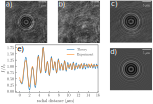
\includegraphics[scale=0.8]{02_body/chapter2/images/lorenz_mie_fit_demo/plot_lorenz_mie.pdf}
		\caption{a) Raw hologram of a $2.5 ~ \mathrm{\mu m}$ polystyrene particle measured experimentaly with the setup detailed in the chapter \ref{chap:exp-setup}. b) Background obtained by taking the mean value of the time series of images of the diffusing particle. c) Normalized hologram given by dividing a) by b). d) Result of the fit of c) using Eq.{\ref{Eq.normalized_Mie}} the particle is found to be at a height $z = 14.77 \mathrm{\mu m}$. e) Comparison of the normalized radial intensity, obtained experimentaly form c) and theoriticaly from d).}
		\label{fig.Lorenz_mie_demo}
\end{figure}


\begin{figure}
	\centering
	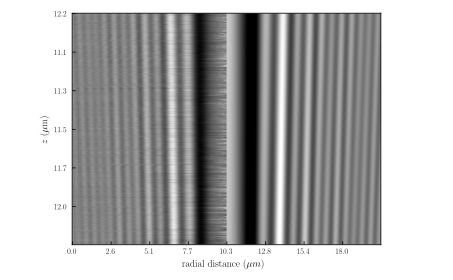
\includegraphics{02_body/chapter2/images/test_tableau2.pdf}
	\caption{On the left, experimentaly measured  holograms' radial intensity stack. Generated from a polysyrene bead (Sigma Aldrich) of nominal radius $a = 1.5 \pm 0.035 \mathrm{\mu m} $ using the experimental setup explained in chapter \ref{chap:exp-setup}. The calibration of this particle radius and optical index is shown in Fig.\ref{fig:KDErn}. On the right, the corresponding theoritical stack using the result of each individual hologram's fit.}
\end{figure}


\subsubsection{ Rayleigh-Sommerfeld back-propagation}





Rayleigh-Sommerfeld back-propagation \cite{wilson_3d_2012} works on the same principle as the Lorenz-Mie fitting but assumes that we have small scatterers.

\begin{equation}
	|\zeta - 1| << 1 \text{ and } ka|\zeta - 1| << 1 ~.
\end{equation}

In this case, at the focal plane, the intensity of the scattered field is smaller than the incident field. Additionaly, the term $|\vec{E}_s|^2$ can be ignored. Thus, the normalized intensity, Eq.\ref{Eq.normalized_Mie} can be rewritten as:

\begin{equation}
	b(\vec{r})= 1 + 2\operatorname{Re}\left( \frac{E_s(\vec{r},0)}{E_0(\vec{r})} \right) ~.
\end{equation}

If you can retrieve completely the scattered field from an image it is possible to reconstruct it above the focal plane by convolution using the Rayleigh-Sommerfeld propagator \cite{goodman_introduction_2005}:

\begin{equation}
	h_{-z}(\vec{r}) = \frac{1}{2 \pi} \frac{\partial}{\partial z} \frac{\mathrm{e}^{ikR}}{R} ~,
	\label{Eq:propagator}
\end{equation}

where $ R^2 = r^2 + z^2 $ and the sign convention on the propagator indicates if the particle is below or above the focal plane. Using this propagator we have:

\begin{equation}
	E_s(\vec{r}, z) = E_z(\vec{r}, 0) \otimes h_{-z}(\vec{r})
\end{equation}

Using the convolution theorem \cite{cheong_strategies_2010, goodman_introduction_2005, sherman_application_1967,schnars_digital_1994} we can write the reconstruted scattered field at a height $z$ by supposing a uniform illumination as:

\begin{equation}
	E_s(\vec{r}, z) \approx \frac{\mathrm{e}^{ikz}}{4\pi ^2}
	\int ^\infty _{- \infty}
	B(\vec{q}) H(\vec{q}, -z) \mathrm{e}^{i \vec{q} \cdot r} d^2 q
	\label{Eq.RS} ~,
\end{equation}

where $B(\vec{q})$ is the Fourier transform of $b(\vec{r})$ and $H(\vec{q}, -z)$ is given by

\begin{equation}
	H(\vec{q}, -z) = \mathrm{e}^{iz \sqrt{k^2 - q^2}} ~.
\end{equation}

Finally, using Eq.\ref{Eq.RS} we can reconstruct the scattered field and intensity since $I(\vec{r}) = |E_s(\vec{r})|^2$ as shown in Fig.\ref{fig.sommerfeld}. 
Those equation are way less computational intensive than the Lorenz-Mie function Eq.\ref{Eq.Lorenz-Mie-function}. Thus tracking can be way faster, moreover, Fourier transforms can be largely accelerated using GPU. Aditionaly, as the propagator Eq.\ref{Eq:propagator} take only into account the intensity of the image, this method does not require any information on the particle and number of particles, here, we just need to assume that we have spherical colloids. Thus this method is great to reconstruct the 3D position of a lot of particles or clusters formations. However, the major drawback is that it is the less precise of the presented measurements and that we can't use it to characterize the particles generating the holograms.

\begin{figure}[h!]
	\centering
	\includegraphics[scale=2]{02_body/chapter2/images/sommerfel_demo.jpg}
	\caption{Figure from \cite{cheong_strategies_2010} a) Volumetric reconstruction using Eq.\ref{Eq.RS} of the scattered intensity de to a single colloidal sphere, colored by intensity. b) Volumetirc reconstructions of $22$ individual $1.58 ~ \mathrm{\mu m}$ diameter silica spheres organised in bcc lattice using holographic optical tweezers in distilled water. Colored regions indicate the isosurface of the brightest 1 percent of reconstructed voxels.}
	\label{fig.sommerfeld}
\end{figure}



\subsubsection{Conclusion}

Finally, the method we choosed is the Lorenz-Mie fitting method, since this method permits the characterization of single particle. Indeed, since we are interested to fine effects near the surface we need to know perfectly the radius of the particle we have recorded. This feature also make our all process, calibration free as we don't need to assume any physical properties. In the following the experimental setup is going to be detailled	.


\subsection{Experimental setup}
\label{chap:exp-setup}
In order to observe the holograms we use an home made inversed microscope as shown on the Fig.\ref{fig:picture} and shematized in Fig.\ref{fig:schema}. A sample consists of a parallelepipedic chamber ($1.5 ~ \text{cm} ~ \times ~ 1.5 ~ \text{cm} ~ \times ~ 150 ~ \mathrm{\mu m} $ ), made from two glass covers, a parafilm spacer, and sealed with vacuum grease, containing a dilute suspension of spherical polystyrene beads. We used 3 differents sizes, of nominal raddi $0.56 ~ \mathrm{\mu m}, ~ 1.5 ~ \mathrm{\mu m} \text{ and } 2.5 ~ \mathrm{\mu m} $, at room temperature $T$, in distilled water (type 1, MilliQ device) of viscosity $\eta = 1 ~ \mathrm{mPa.s}$. The sample is illuminated by a collimated laser beam with a $521 ~ \mathrm{\mu m}$ wavelength. The explain in the chapter 3.3..., the light scattered by one colloidal particle at a given time $t$ interferes with the incident beam. An oil-immersion objective lens (x60 magnification, $1.30$ numerical aperture) collects the ersulting instantaneous interference pattern, and relays it to a camera (Basler acA1920-155um) with a $51.6$ nm/pixel resolution (see Fig.\ref{fig.Lorenz_mie_demo}a)). The exposure time of the camera is set to $3$ ms to avoid motion-induced blurring of the image, as a general rule, the particle should not diffuse more than the pixel size during that time.

\begin{figure}[h!]
	\centering
	\includegraphics{02_body/chapter2/images/figures_setup/photo_setup.pdf}
	\caption{Photo of the custom build microscope used along my thesis. It is mainly composed of Thorlabs cage system. The camera used is a Basler acA1920-155um, we use a x60 magnification and $1.30$ numerical aperture oil immersion objective and the laser is colimated and has a $521 \mathrm{\mu m}$ wavelength.}
	\label{fig:picture}
\end{figure}

\begin{figure}[h!]
	\centering
	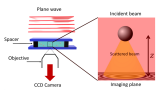
\includegraphics[scale=0.9]{02_body/chapter2/images/figures_setup/schema_setup.pdf}
	\caption{Schematic of the experimental setup. A lase plane wave of intensity $E_0$ illuminates the chamber containing a dilute suspension of microspheres in water. The light scattered by a particle interferes with the incident beam onto the focal plane of an objective lens, that magnifies the interference patten and relays it to a camera.}
	\label{fig:schema}
\end{figure}


\subsection{Hologram fitting strategy}

\subsubsection{How to fasten the process ?}

As presented in the section \ref{chap:LM_fit} about the Lorenz-Mie fitting. The main drawback is the time to fit an image, from $30$ seconds for the images of $100 \times  100$ pixels to a few minutes for the $500\times 500$ pixels. We can directly see a bottleneck, indeed, if we want to track one trajectory made of $100~000$ images we would need to wait $\approx 70$ days for a series of images that need only a few minutes to be shot experimentaly. When I started my PhD, two groups, the Grier's lab and the Manoharan's lab, had already introduced python packages, respectively, Pylorenzmie and Holopy in order to inverse holograms. They had introduce ways to only fit a set of randomly choosen pixels and demonstrated that taking only $1\%$ of the image pixel could lead to similar precision and improve considerably the fits \cite{dimiduk_random-subset_2014}. Unfortunatly, even if this is faster, it leads to a few images per second and still is too long for the amount of data we wanted to have. Ironicaly, this part of my project is certainly the one I spent the most time, and learn a lot of things on code optimization and computer cluster usage. It's around the half of my thesis that Pylorenzmie got a new commit on their github repository which was telling that they succeeded on using GPU acceleration using CUDA. This was not an easy task since they needed to reconstruct the Bessel, fortunatly it is possible by using continued fractions \cite{lentz_generating_1976}. This tiny update permits to fit whole images at a whooping speed improvment of 20 fps. At this, speed we fit the tridimension position of the particle, the radius and optical index. To have a more reliable and fast tracking what we do is that we will fit with all free parameters the first $10~000$ of a movie and determine the physical properties of the colloidal particle and then fit the whole movie with only the position as a free parameter.

\subsubsection{Radius and optical index characterization}


Once the data of the radius and optical index retrieved, the first quantity we can look at the the distribution of measurements. Using our $10 ~ 000$ measurements we can plot the histograms of the measured $a$ and $n_\mathrm{p}$.




This simple histogram could suffice to meausure the physical properties of the colloidal particle. However, we can go a bit further and look at the 2D histogram of the $a$ and $n_\mathrm{p}$ as presented in the fig.XX here smoothed using a Gaussian kernel density estimator. Ae we can see it is not isotropic and it seems that the measurement of $n_\mathrm{p}$ and $a$ are correlated.
 

\begin{figure}[h!]
	\centering
	\includegraphics{02_body/chapter2/images/KDErn.pdf}
	\caption{2D Probability density function of the measurements of the optical index $n_\mathrm{p}$ and radius $a$. Black lines indicates iso-probability. Taking the $10\% $ top probability, we measure $n_\mathrm{p} = 1.585 \pm 0.002$ and $a=1.514 \pm 0.003 ~ \mathrm{\mu m}$. }
	\label{fig:KDErn}
\end{figure}